\documentclass[UTF8,a4paper,11pt,fontset=fandol]{ctexart}
\usepackage[margin=2.3cm]{geometry}
\usepackage{amsmath,amssymb,booktabs,tabularx,array,enumitem}
\usepackage{xcolor,listings,tikz,placeins,needspace,graphicx}
\usetikzlibrary{arrows.meta,positioning}
\usepackage{gbt7714}
\bibliographystyle{gbt7714-numerical}
\usepackage[hidelinks]{hyperref}
\usepackage{xurl}
\newcommand{\code}[1]{\nolinkurl{#1}}
\newcolumntype{Y}{>{\raggedright\arraybackslash}X}
\newcommand{\Kn}{\mathit{Kn}}
\setlength{\parskip}{0.25em}
\setlength{\emergencystretch}{2em}
\clubpenalty=10000
\widowpenalty=10000
\linespread{1.16}
\setlist{leftmargin=2em,itemsep=0.2em,topsep=0.3em}
\ctexset{section={beforeskip=1.4ex,afterskip=0.8ex},subsection={beforeskip=1ex,afterskip=0.5ex}}
\definecolor{codebg}{RGB}{247,248,250}
\lstset{basicstyle=\ttfamily\small,backgroundcolor=\color{codebg},frame=single,
rulecolor=\color{black!20},breaklines=true,columns=fullflexible,keepspaces=true,
showstringspaces=false,xleftmargin=0.3em,xrightmargin=0.3em}
\tikzset{box/.style={draw=black!55,fill=blue!3,align=center,text width=39mm,
minimum height=12mm,font=\small},flow/.style={-{Stealth[length=2mm]},thick}}
\tikzset{
restrictionline/.style={-{Stealth[length=1.2mm]},line width=0.7pt,draw=blue!70!black},
prolongationline/.style={-{Stealth[length=1.2mm]},line width=0.7pt,dashed,draw=red!70!black}
}
\newcommand{\cycleplot}[3]{%
\foreach \y in {0,1,2,3}{\draw[dotted,gray!60] (0,\y)--(#3,\y);}
\xdef\prevlevel{-1}
\foreach \lev [count=\i from 0] in {#1}{%
\pgfmathsetmacro{\xx}{\i*#2}
\coordinate (p\i) at (\xx,\lev);
\ifnum\i>0
\pgfmathtruncatemacro{\j}{\i-1}
\ifnum\lev<\prevlevel
\draw[restrictionline] (p\j)--(p\i);
\else
\draw[prolongationline] (p\j)--(p\i);
\fi
\fi
\xdef\prevlevel{\lev}
}
\foreach \lev [count=\i from 0] in {#1}{%
\pgfmathsetmacro{\xx}{\i*#2}
\ifnum\lev=0
\fill (\xx,\lev) circle[radius=1.5pt];
\else
\draw[fill=white] (\xx,\lev) circle[radius=1.5pt];
\fi
}
}
\begin{document}
\pagestyle{plain}
\begin{center}
{\LARGE\bfseries HyMoS\par}
\vspace{0.5em}
{\large 北太天元插件开发技术文档\par}
\vspace{0.6em}
{\small  2026 年 10 月}
\end{center}
\noindent 本项目面向 B3“自选开源库插件开发”，将 HyMoS（Hyperbolic Moment Solver）接入北太天元，采用快速迭代矩方法（FIM）求解一维稳态玻尔兹曼方程的 BGK 模型，支持 Couette、Fourier 及 Couette--Fourier 平行板流动。插件通过图形界面配置计算，提供运行监视、结果分析和数据导出。

\section{开发背景}
HyMoS 是面向稳态气体动理学计算的 C++ 求解库，其特点是将可调阶数的双曲矩模型、快速稳态迭代和可配置求解流程集成于同一计算核心。BGK 模型以弛豫项近似分子碰撞\cite{bgk1954}，Grad 矩方法以有限个矩描述分布函数\cite{grad1949}，全局双曲正则化为任意阶矩系统提供了统一的闭合形式\cite{cai2014}。用户可通过矩阶数 $M$ 调整分布函数的近似层次，在宏观守恒量之外保留应力、热流等非平衡信息。

选用 HyMoS 的主要依据是其面向近连续流域的稳态求解能力。快速迭代矩方法（FIM）交替更新高阶矩系统及相容的流体力学子系统，利用宏观方程加速密度、速度和温度的收敛\cite{li2026}；Hu 和 Li 提出的非线性多重网格方法（NMG）通过空间粗网格校正进一步加速稳态迭代\cite{hu2014}。HyMoS 将二者组合，提供三种 FIM 配置及 V/F/W 循环，适合在统一模型下比较矩阶数、网格和求解策略。

HyMoS 的算例和求解配置相互独立，网格、壁面条件及迭代参数可在运行时设置。这一结构便于将已有求解器封装为共享库，复用同一计算核心完成三类平行板流动计算，并通过内存接口向宿主返回场量及残差记录。插件开发可集中于宿主接口、任务管理和交互设计，同时保持求解过程及数值格式的一致性。

接入北太天元后，插件提供一维稳态 BGK 方程的专用求解能力，并将参数配置、任务控制和结果分析组织为连续操作流程。用户在原生图形界面中设置工况，计算结果直接进入北太天元工作区，可继续用于绘图、数组运算及不同工况的对比分析；输入快照和结果导出则保留每次计算的条件及输出，便于复核。

工业应用可聚焦于微机电系统的气体薄膜和微尺度间隙，平行板流动是分析其稀薄输运效应的基础模型\cite{cercignani2006}。本插件的 Couette 工况可用于考察平行壁面相对运动引起的气体剪切，Fourier 工况可用于分析温差驱动的间隙传热，耦合工况可用于研究剪切和传热的相互影响。通过改变 $\Kn$、壁速及壁温，可获得速度、温度和热流分布，为近似平行间隙的气体阻力、传热特性评估及设计参数筛选提供计算依据。
\section{算法原理}
\subsection{动理学模型}
无外力 Boltzmann--BGK 方程表示为
\begin{equation}
\frac{\partial f}{\partial t}
+\boldsymbol\xi\cdot\nabla_{\boldsymbol x}f
=\bar\nu(f^M-f),
\qquad
f^M=\frac{\rho}{m_*(2\pi\theta)^{3/2}}
\exp\!\left(-\frac{|\boldsymbol\xi-\boldsymbol u|^2}{2\theta}\right).
\end{equation}
其中 $f=f(t,\boldsymbol x,\boldsymbol\xi)$ 为分子分布函数，$t$ 为时间，$\boldsymbol x\in\mathbb R^3$ 为位置，$\boldsymbol\xi\in\mathbb R^3$ 为分子速度；$\bar\nu$ 为碰撞频率，$m_*$ 为单个分子的质量。局部 Maxwell 分布 $f^M$ 由密度 $\rho$、平均速度 $\boldsymbol u$ 和温度变量 $\theta$ 确定，其定义为
\begin{equation}
\begin{aligned}
\rho&=m_*\int_{\mathbb R^3}f\,\mathrm d\boldsymbol\xi,
&\rho\boldsymbol u&=m_*\int_{\mathbb R^3}\boldsymbol\xi f\,\mathrm d\boldsymbol\xi,\\
\rho|\boldsymbol u|^2+3\rho\theta
&=m_*\int_{\mathbb R^3}|\boldsymbol\xi|^2f\,\mathrm d\boldsymbol\xi.
\end{aligned}
\end{equation}

插件采用无量纲形式，流动仅沿壁面法向 $x_1$ 变化。稳态下 $\partial_t f=\partial_{x_2}f=\partial_{x_3}f=0$，上述方程化为
\begin{equation}
\xi_1\frac{\partial f}{\partial x_1}=\bar\nu(f^M-f),
\qquad
\bar\nu=\sqrt{\frac{\pi}{2}}\frac{\rho\theta^{1-\omega}}{\Kn},
\quad \omega=0.81.
\end{equation}
此时 $f=f(x_1,\boldsymbol\xi)$，物理空间为一维，分子速度仍保留三个分量。模型取 $\mathrm{Pr}=1$，两壁采用完全漫反射边界，壁温和切向速度由用户设置。

\subsection{快速迭代矩方法（FIM）}
HyMoS 将分布函数按局部 Hermite 基展开并截断至 $M$ 阶，经全局双曲正则化得到闭合矩系统，再采用有限体积法离散物理空间\cite{cai2014,cai2010}。FIM（fast iterative moment method）交替求解矩系统及相容的流体力学子系统：先更新高阶矩并计算应力、热流，再以这些量闭合宏观方程，更新密度、速度和温度，最后将宏观量回代矩系统，直至残差满足容差\cite{li2026,lidoctor2026}。

三种 FIM 配置采用的更新格式见表\ref{tab:fim-configurations}。
\begin{table}[htbp]
\centering\small
\caption{FIM 求解配置}\label{tab:fim-configurations}
\begin{tabularx}{0.9\textwidth}{@{}p{23mm}YY@{}}
\toprule
求解器 & 高阶矩系统 & 流体力学子系统\\
\midrule
FIM-1 & 显式 Euler & 显式 Euler\\
FIM-2 & IMEX & 显式 Euler\\
FIM-3 & IMEX-SGS & SGS\\
\bottomrule
\end{tabularx}
\par\smallskip
\begin{minipage}{0.9\textwidth}\footnotesize
IMEX：输运项显式、碰撞项隐式；SGS：对称 Gauss--Seidel 扫掠。
\end{minipage}
\end{table}
\FloatBarrier

\subsection{非线性多重网格方法（NMG）}
NMG（nonlinear multigrid）通过空间粗网格校正加速稳态求解\cite{hu2014}。插件以 FIM 为各层网格的光滑子，将细网格近似解和残差限制到粗网格，计算校正后传回细网格；各层保持相同矩阶数 $M$。界面中的 \code{single} 对应单网格 FIM，\code{nmg} 对应上述组合方法，可设置最粗网格尺寸、光滑步数及 V/F/W 循环，路径见图\ref{fig:nmg-cycles}。


\begin{figure}[htbp]
\centering
\begin{minipage}[b]{0.31\textwidth}
\centering
\begin{tikzpicture}[x=1cm,y=0.62cm]
\path[use as bounding box] (-1.1,-0.35) rectangle (2.7,3.35);
\node[anchor=east,font=\scriptsize] at (-0.13,3) {最细层};
\node[anchor=east,font=\scriptsize] at (-0.13,0) {最粗层};
\cycleplot{3,2,1,0,1,2,3}{0.45}{2.70}
\end{tikzpicture}
\par\smallskip{\small (a) V 循环}
\end{minipage}\hfill
\begin{minipage}[b]{0.31\textwidth}
\centering
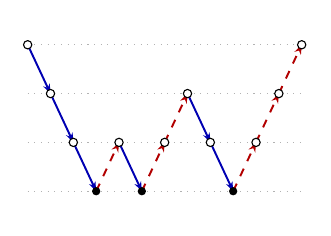
\begin{tikzpicture}[x=1cm,y=0.62cm]
\path[use as bounding box] (0,-0.35) rectangle (3.5,3.35);
\cycleplot{3,2,1,0,1,0,1,2,1,0,1,2,3}{0.29}{3.48}
\end{tikzpicture}
\par\smallskip{\small (b) F 循环}
\end{minipage}\hfill
\begin{minipage}[b]{0.31\textwidth}
\centering
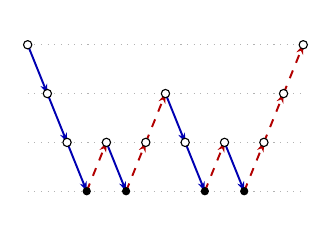
\begin{tikzpicture}[x=1cm,y=0.62cm]
\path[use as bounding box] (0,-0.35) rectangle (3.5,3.35);
\cycleplot{3,2,1,0,1,0,1,2,1,0,1,0,1,2,3}{0.25}{3.50}
\end{tikzpicture}
\par\smallskip{\small (c) W 循环}
\end{minipage}
\par\medskip
{\footnotesize
\tikz[baseline=-0.5ex]\draw[fill=white] (0,0) circle[radius=1.5pt];\ 光滑
\quad
\tikz[baseline=-0.5ex]\fill (0,0) circle[radius=1.5pt];\ 最粗层求解
\quad
\tikz[baseline=-0.5ex]\draw[restrictionline] (0,0)--(0.45,0);\ 限制
\quad
\tikz[baseline=-0.5ex]\draw[prolongationline] (0,0)--(0.45,0);\ 延拓
}
\caption{NMG 循环示意。图示采用四层网格，同层连续操作合并为一个节点。}
\label{fig:nmg-cycles}
\end{figure}
\FloatBarrier
\Needspace{32\baselineskip}
\section{插件设计}
\subsection{模块结构}
插件由宿主交互、SDK 适配、任务引擎和数值求解四个模块组成，调用关系见图\ref{fig:architecture}。任务引擎及数值求解器封装于 HyMoS 共享库，北太天元通过 SDK 适配模块调用该库\cite{sdk}。
\begin{figure}[htbp]
\centering
\begin{tikzpicture}[
module/.style={draw=black!55,fill=blue!3,align=center,text width=116mm,
minimum height=13mm,font=\small,inner sep=3mm},
request/.style={-{Stealth[length=1.8mm]},line width=0.8pt,draw=blue!70!black},
response/.style={-{Stealth[length=1.8mm]},line width=0.8pt,dashed,draw=black!65},
edgecaption/.style={font=\scriptsize,fill=white,inner sep=1.5pt}]
\draw[rounded corners=2mm,draw=black!35,fill=green!2] (-6.8,-8.25) rectangle (6.8,-3.55);
\node[anchor=north,font=\small\bfseries] at (0,-3.68) {HyMoS 共享库\quad\texttt{libhymos.so.5}};
\node[module] (host) at (0,0) {\textbf{宿主交互模块}\quad 北太天元 M 脚本\\参数表单、配置加载保存、运行监视、结果绘图};
\node[module] (adapter) at (0,-2.3) {\textbf{SDK 适配模块}\quad\texttt{main.so}\\函数注册、任务句柄、宿主数据转换、CSV 导出};
\node[module,fill=green!4] (engine) at (0,-5.05) {\textbf{任务引擎}\\参数校验、输入快照、后台线程、进度记录};
\node[module,fill=green!4] (solver) at (0,-7.25) {\textbf{数值求解器}\\Hermite 矩离散、平行板边界、FIM 迭代、NMG 校正};
\draw[request] ([xshift=-30mm]host.south)--node[edgecaption,left]{参数、运行指令} ([xshift=-30mm]adapter.north);
\draw[response] ([xshift=30mm]adapter.north)--node[edgecaption,right]{状态、结果结构体} ([xshift=30mm]host.south);
\draw[request] ([xshift=-30mm]adapter.south)--node[edgecaption,left]{提交、查询、停止} ([xshift=-30mm]engine.north);
\draw[response] ([xshift=30mm]engine.north)--node[edgecaption,right]{任务状态、结果数组} ([xshift=30mm]adapter.south);
\draw[request] ([xshift=-30mm]engine.south)--node[edgecaption,left]{计算配置、停止标记} ([xshift=-30mm]solver.north);
\draw[response] ([xshift=30mm]solver.north)--node[edgecaption,right]{迭代进度、场量} ([xshift=30mm]engine.south);
\end{tikzpicture}
\caption{插件模块及数据流。实线为配置及控制传递，虚线为状态及结果返回。}
\label{fig:architecture}
\end{figure}
\FloatBarrier

本项目将左右壁温及切向壁速参数化，通过统一求解入口支持 Couette、Fourier 及耦合工况。任务引擎在提交时校验参数、保存输入快照并创建独立任务目录，随后启动后台求解线程；适配模块在宿主调用时读取进度，并将结果复制为北太天元结构体及列主序数组，供脚本分析和绘图。

插件每次执行一个计算任务。界面应用后的配置用于下一次提交，已启动的任务按其输入快照计算。停止请求通过共享标记传入求解器，在迭代检查点生效；释放最后一个任务引用或卸载插件时，先请求停止，再等待工作线程退出。输入快照、分布展开数据和导出结果保存在对应任务目录。

\subsection{技术栈}
\begin{center}\small
\begin{tabularx}{\textwidth}{@{}p{26mm}p{45mm}Y@{}}
\toprule
模块 & 主要技术 & 用途\\
\midrule
宿主交互 & M 语言、原生 \texttt{uifigure} & 构建分类参数窗口，调用宿主绘图及工作区功能。\\
SDK 适配 & C++11、北太天元 SDK & 注册插件函数，管理任务句柄，转换输入及结果数据。\\
任务引擎 & C++11 线程、原子变量 & 后台执行、进度同步及协作停止。\\
数值求解 & C++11、OpenMP & 实现矩方法、FIM/NMG 迭代及数值计算并行。\\
工程构建 & CMake、GNU C++ & 构建共享库及插件，组织脚本、模板和算例打包。\\
\bottomrule
\end{tabularx}
\end{center}
第三方依赖及构建环境见部署方法。
\Needspace{13\baselineskip}
\section{部署方法}
\subsection{插件安装}
预编译包可直接安装使用，内含 HyMoS 求解库、界面脚本、配置模板和算例。本文部署环境为 Ubuntu 24.04.4 LTS（WSL2）及北太天元 2025 Linux 版，界面使用北太天元原生组件。

GNU C/C++ 及 OpenMP 运行库由系统提供；OpenMP 运行库可通过 \texttt{sudo apt install libgomp1} 安装。Eigen、Boost、MPI、FFTW 和 oneTBB 用于源码构建，使用预编译包无需另行安装。

从项目发布页下载预编译包，解压后将完整的 \code{HyMoS/} 目录放入北太天元的 \code{plugins/} 目录，保留根目录的 \code{main.so} 及 \code{lib/}、\code{ui/}、\code{assets/}、\code{examples/}。同一会话加载一个 HyMoS 版本，更换版本后重启宿主。任务输出默认位于 \code{/tmp/hymos_baltamatica_runs}；如需长期保存，可在启动宿主前通过 \code{HYMOS_RUNS_ROOT} 指定用户可写目录。

\subsection{源码构建（开发者可选）}
源码构建用于修改程序后重新生成插件，或复现开发测试；直接使用预编译包时可跳过本节。工程采用 C++11、CMake、OpenMP 和北太天元 SDK，已验证编译工具为 GNU C++ 9.5.0、CMake 3.28.3。下表列出工程默认构建配置使用的第三方依赖。
\begin{center}\small
\begin{tabularx}{\textwidth}{@{}p{22mm}p{19mm}Y@{}}
\toprule
依赖 & 核对版本 & 获取地址\\
\midrule
Eigen & 3.4.0 & \url{https://gitlab.com/libeigen/eigen}\\
Boost & 1.83 & \url{https://www.boost.org}\\
Open MPI & 4.1.6 & \url{https://www.open-mpi.org}\\
FFTW & 3.3.10 & \url{https://www.fftw.org}\\
oneTBB & 2021.11.0 & \url{https://github.com/uxlfoundation/oneTBB}\\
\bottomrule
\end{tabularx}
\end{center}
\Needspace{12\baselineskip}
安装北太天元 SDK 后，在 Ubuntu 中安装开发依赖，并于源码根目录执行以下命令，其中 Python 3 用于测试脚本。
\begin{lstlisting}
sudo apt install build-essential cmake python3 libopenmpi-dev \
  libeigen3-dev libboost-serialization-dev libboost-system-dev \
  libboost-thread-dev libfftw3-dev libtbb-dev
bash scripts/build.sh --prefix /opt/Baltamatica
\end{lstlisting}
构建脚本自动执行回归测试，结果位于 \code{build-release/plugin/HyMoS/}。可按第 4.1 节复制安装，或执行 \lstinline|bash scripts/install.sh --prefix /opt/Baltamatica|。

\Needspace{26\baselineskip}
\section{操作流程}
\subsection{设置参数}
输入文件采用 INI 格式，按方括号中的节名组织参数。物理量均采用无量纲形式，各节含义如下。
\begin{itemize}[label={},leftmargin=0pt,itemsep=0.25em]\raggedright
\item \textbf{\texttt{[System]}}：\code{Temperature} 为参考温度；\code{ORDER} 为矩阶数 $M$；\code{n_thread} 为计算线程数，建议取 1--4。
\item \textbf{\texttt{[Mesh]}}：\code{Nx} 为网格单元数 $N_1$，最小为 8；\code{L0} 为区间左端点；\code{Len} 为区间长度。
\item \textbf{\texttt{[Time]}}：\code{CFL}、\code{CFL_HEs} 分别控制矩系统及流体力学子系统的时间步长。
\item \textbf{\texttt{[Const]}}：\code{Kn} 为 Knudsen 数。
\item \textbf{\texttt{[Error]}}：\code{Tol} 为稳态残差容差。
\item \textbf{\texttt{[Solver]}}：\code{SolverType} 取 \code{single} 或 \code{nmg}；\code{FIM} 取 1、2、3，对应表\ref{tab:fim-configurations}中的配置。
\item \textbf{\texttt{[SingleGridMethod]}}：\code{EulerEqsSolvingSteps} 为每轮 FIM 中流体力学子系统的最大迭代步数。
\item \textbf{\texttt{[MultiGridMethod]}}：\texttt{PreSmoothingSteps}、\texttt{PostSmoothingSteps} 为前、后光滑次数；\texttt{CoarsestGridSmoothingSteps} 为最粗层光滑次数；\texttt{CoarsestGridSize} 为最粗网格单元数。\code{CycleType} 取 1、2、3，分别对应 V、W、F 循环。各层网格逐次二分。
\item \textbf{\texttt{[LeftWall]}}、\textbf{\texttt{[RightWall]}}：分别设置左右壁面的 \code{Temperature}（壁温）和 \code{TangentialVelocity}（沿 $u_2$ 方向的切向壁速）。
\end{itemize}

\Needspace{22\baselineskip}
以下为 Couette 工况的 input 参数示例，采用 FIM-3 和 NMG，按左、右两栏顺序展示。固定项沿用随包模板，在模板上按下例修改。
\par\smallskip
\noindent
\begin{minipage}[t]{0.48\textwidth}
\vspace{0pt}
\begin{lstlisting}[basicstyle=\ttfamily\small\linespread{1}\selectfont]
[System]
Temperature = 1
ORDER = 7
n_thread = 4

[Mesh]
Nx = 128
L0 = -0.5
Len = 1.0

[Time]
CFL = 0.8
CFL_HEs = 0.8

[Const]
Kn = 0.01

[Error]
Tol = 1e-8
\end{lstlisting}
\end{minipage}\hfill
\begin{minipage}[t]{0.48\textwidth}
\vspace{0pt}
\begin{lstlisting}[basicstyle=\ttfamily\small\linespread{1}\selectfont]
[Solver]
SolverType = nmg
FIM = 3

[SingleGridMethod]
EulerEqsSolvingSteps = 600

[MultiGridMethod]
PreSmoothingSteps = 2
PostSmoothingSteps = 2
CoarsestGridSmoothingSteps = 4
CoarsestGridSize = 8
CycleType = 1

[LeftWall]
Temperature = 1.0
TangentialVelocity = -0.62885

[RightWall]
Temperature = 1.0
TangentialVelocity = 0.62885
\end{lstlisting}
\end{minipage}
\par\smallskip

\Needspace{34\baselineskip}
上述参数也可在图形界面中直接填写。加载插件并打开配置窗口：
\begin{lstlisting}
load_plugin('HyMoS');
hymos_setup('1D');
\end{lstlisting}
图\ref{fig:plugin-parameters}展示参数窗口的“物理参数”页。在左侧依次选择“物理参数”“网格与阶数”“求解方法”，填写对应参数；求解方法选为 \code{nmg} 后，可编辑“多重网格”设置。点击“检查参数”，通过后点击“应用并关闭”。“加载参数”可读取随包的 \code{couette.txt}、\code{fourier.txt} 和 \code{couette_fourier.txt}；“保存参数”或“另存为”用于保存完整配置。
\begin{figure}[htbp]
\centering
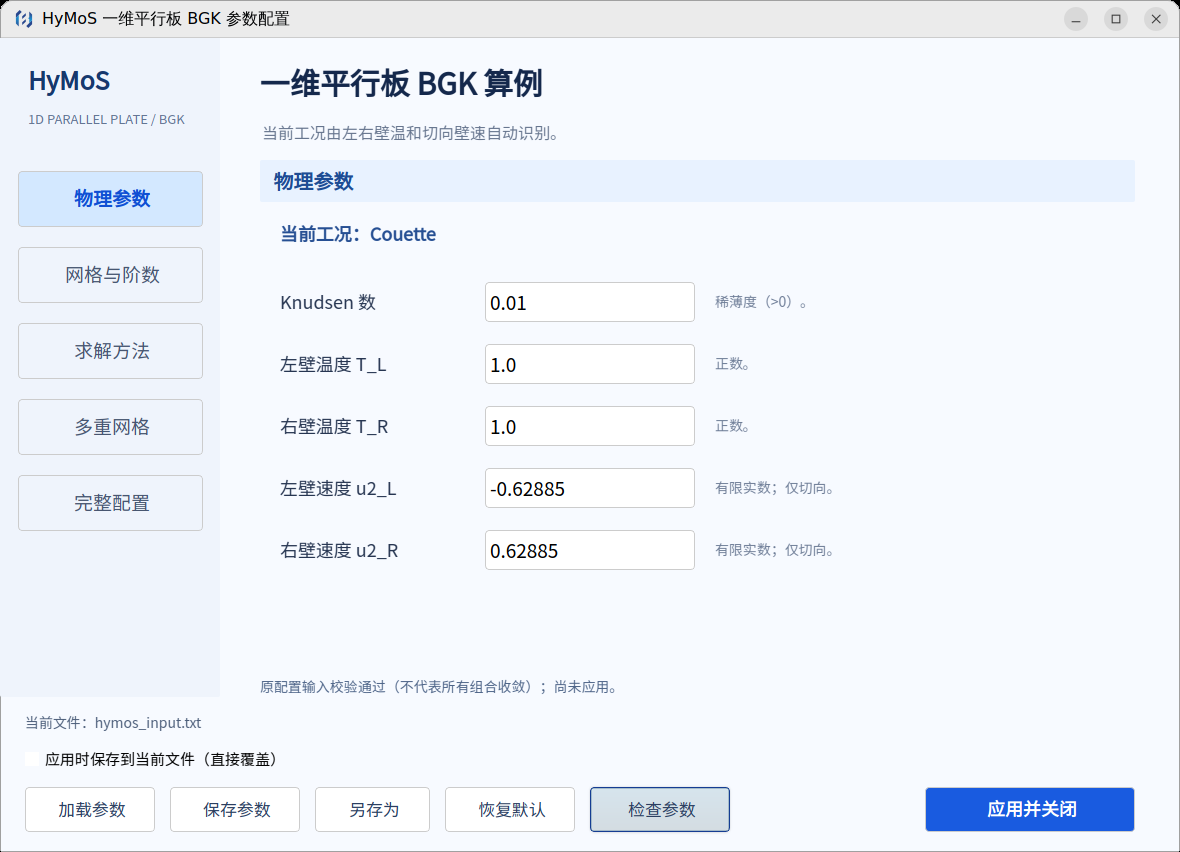
\includegraphics[width=\textwidth]{figures/plugin_parameters.png}
\caption{插件参数窗口。左侧切换参数分类，底部完成加载、保存、检查及应用。}
\label{fig:plugin-parameters}
\end{figure}
\FloatBarrier

\Needspace{9\baselineskip}
\subsection{启动计算}
在命令窗口执行：
\begin{lstlisting}
hymos_run();
\end{lstlisting}
该命令使用已应用的界面参数启动计算，将任务保存为工作区变量 \code{hymos_task}，并显示状态、迭代数、残差和耗时。状态 \code{converged} 表示残差达到容差，\code{iteration_limit} 表示达到迭代上限。

\Needspace{13\baselineskip}
\subsection{运行控制}
运行中按 Ctrl+C 可中断前台监视并返回命令窗口，后台计算继续。表\ref{tab:control}列出常用控制调用，其中 \code{hymos_task} 为当前任务对象。
\begin{table}[htbp]
\centering\small
\caption{任务控制接口}\label{tab:control}
\begin{tabularx}{\textwidth}{@{}p{0.48\textwidth}Y@{}}
\toprule
调用 & 功能及返回值\\
\midrule
\code{s=hymos_status(hymos_task)} & 查询任务，返回状态、迭代数、残差及耗时等。\\
\code{hymos_monitor(hymos_task)} & 继续监视，默认每 0.5 秒刷新。\\
\code{hymos_stop(hymos_task)} & 请求安全停止；生效后状态变为 \code{stopped}。\\
\code{s=hymos_wait(hymos_task,10)} & 等待任务结束或 10 秒超时，返回任务状态。\\
\bottomrule
\end{tabularx}
\end{table}
\FloatBarrier
任务结束后，可读取已有场量并导出计算结果。

\subsection{查看结果}
任务收敛后，读取结果、绘制温度曲线并导出。图\ref{fig:plugin-temperature}展示北太天元中的绘图窗口。
\begin{lstlisting}
r = hymos_result(hymos_task);
plot(r.x, r.temperature);
xlabel('x', 'Interpreter', 'none');
ylabel('Temperature', 'Interpreter', 'none');
files = hymos_export(hymos_task);
\end{lstlisting}
\code{r} 为结果结构体，包含坐标、密度、三分量速度、温度、二阶矩系数、热流、残差历史和运行信息；常用字段为 \code{x}、\code{density}、\code{velocity}、\code{temperature}、\code{heat_flux} 及 \code{residual}。\code{stress_moments} 保存三个二阶 Hermite 系数 $f_{2\hat e_1}$、$f_{\hat e_1+\hat e_2}$、$f_{2\hat e_2}$，其中 $\hat e_i$ 为单位多重指标。

\code{files} 返回导出路径。场量、残差和元数据分别保存为 \code{couette_fields.csv}、\code{residual.csv} 和 \code{result_metadata.txt}；任务目录同时保留 \code{input.resolved.txt} 输入快照及 \code{DisSol1th.dat} 分布展开数据，便于复核计算条件。
\begin{figure}[htbp]
\centering
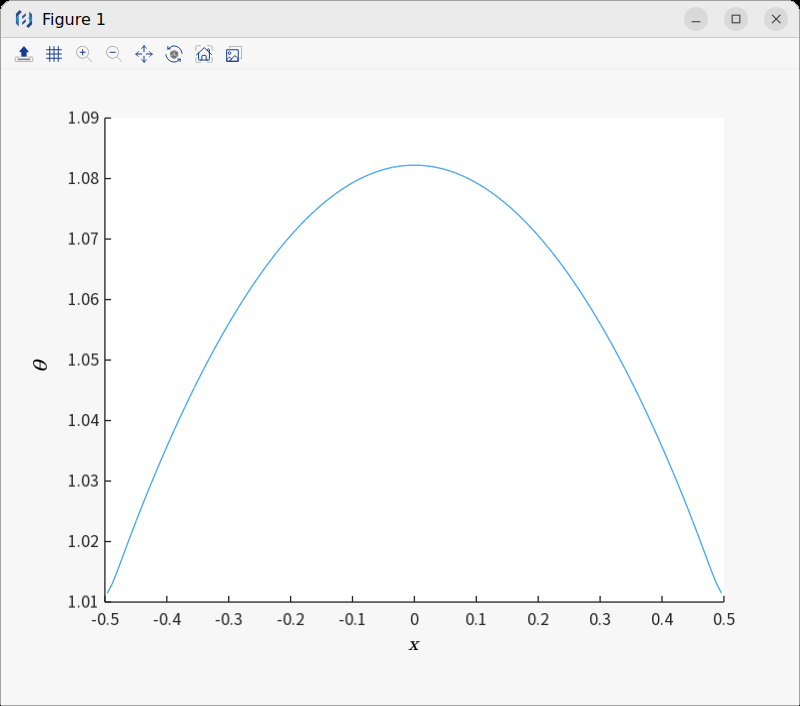
\includegraphics[width=0.74\textwidth]{figures/plugin_temperature.png}
\caption{Couette 工况的温度曲线。由北太天元绘制。}
\label{fig:plugin-temperature}
\end{figure}

\FloatBarrier

\section{项目资料}
公开仓库：\url{https://github.com/Liuyong2355/HyMoS}。源码、编译后的插件、技术文档、接口参考、测试源码及演示视频统一在仓库和发布页提供。第三方依赖的来源和许可见仓库中的 \code{THIRD_PARTY_NOTICES.md}。

图形界面借助 AI 辅助开发，技术文档借助 AI 整理，演示视频借助 AI 剪辑。

{\small\linespread{1}\selectfont
\setlength{\bibsep}{0.3em}
\bibliography{references}
}
\end{document}